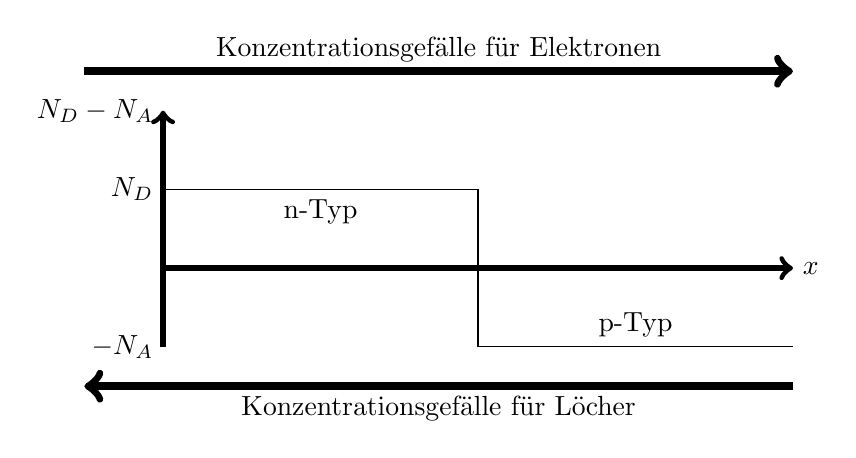
\begin{tikzpicture}
%Achsen
  \draw[line width=2pt,->] (0,0) -- (0,3);
  \draw (0,3) node
    [anchor=east]
    {$N_D - N_A$};
  \draw[line width=2pt,->] (0,1) -- (8,1);
  \draw (8,1) node
    [anchor=west]
    {$x$};
%Gefälle
  \draw[line width=3pt,->] (-1,3.5) -- (8,3.5);
  \draw (3.5,3.5) node
    [anchor=south]
    {Konzentrationsgefälle für Elektronen};
  \draw[line width=3pt,->] (8,-0.5) -- (-1,-0.5);
  \draw (3.5,-0.5) node
    [anchor=north]
    {Konzentrationsgefälle für Löcher};
%Graph
  \draw (0,2) node
    [anchor=east]
    {$N_D$};
  \draw (0,0) node
    [anchor=east]
    {$-N_A$};
  \draw (0,2) -- (4,2);
  \draw (2,2) node
    [anchor=north]
    {n-Typ};
  \draw (4,2) -- (4,0);
  \draw (4,0) -- (8,0);
  \draw (6,0) node
    [anchor=south]
    {p-Typ};
\end{tikzpicture}

